\documentclass{article}
\usepackage{amsmath, amssymb, amsfonts}
\usepackage{tikz}
\usepackage{filecontents}
\usepackage{listings}
\usepackage{stmaryrd}
\usepackage[margin=1in]{geometry}
\usepackage{amsthm}
\long\def\/*#1*/{}

\lstdefinestyle{base}{
  emptylines=1,
  breaklines=true,
  basicstyle=\ttfamily\color{black},
  basicstyle=\footnotesize\ttfamily,
  moredelim=**[is][\color{red}]{@}{@},
}

\swapnumbers
\theoremstyle{plain}
\theoremstyle{definition}
\newtheorem{defn}{Definition}

\usetikzlibrary{arrows}
\begin{document}
\noindent



\section{Two operational semantics for Soft Component System}
\subsection{Soft Component Automata}
\paragraph{Syntax} Syntax. \\
State and transition, semiring values and component actions.

\paragraph{Example} Example. \\
East West patrolling agent.

\begin{filecontents*}{temp.tikz}
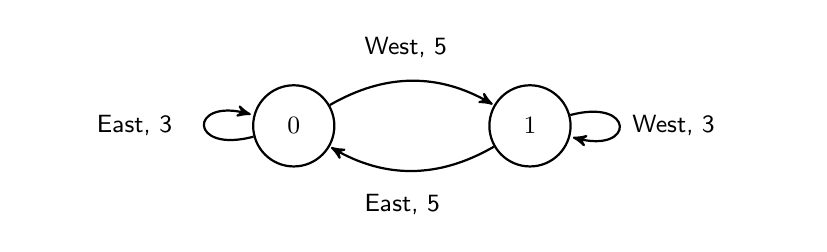
\begin{tikzpicture}[->,>=stealth',shorten >=0.5pt,auto,node distance=3cm,
                    thick,main node/.style={circle,draw,font=\sffamily\small}, align=center, text width=2cm]

  \node[main node, text width=0.7cm] (1) {$0$};
  \node[main node, text width=0.7cm] (2) [right of=1] {$1$};

  \node[align=left,font=\sffamily\small] (A) at (-1.5,0) {East, 3};
  \node[align=left,font=\sffamily\small] (B) at (5.3,0) {West, 3};
  \node[align=left,font=\sffamily\small] (D) at (1.9,1) {West, 5};
  \node[align=left,font=\sffamily\small] (E) at (1.9,-1) {East, 5};
  \path[every node/.style={font=\sffamily\small}]
    (1) edge [bend left] node [above,sloped] {} (2)
        edge [loop left] node { } (1)
    (2) edge [bend left] node [below,sloped] {} (1)
        edge [loop right] node { } (2);
\end{tikzpicture}
\end{filecontents*}
\begin{figure}[htb]
\centering
\resizebox{9cm}{!}{ \begin{tikzpicture}[>=latex,shorten >=1pt,node distance=3cm,on grid,auto, node/.style={circle,draw,minimum size=25pt}, ]

 \node[state] (B) at (80pt,0pt) {$s_1$};

 \node[state] (A) at (0pt,0pt) {$s_0$};
 \draw[<-] (A) -- node[above left] {} ++(-1,0);
 \draw[->] (B) to[out=20,in=-20,looseness=8] node[right, align=left] {pass, 1} (B);
 \draw[->] (A) to[out=20,in=160,looseness=1] node[above] {snapshot, 0} (B);
 \draw[->] (B) to[out=200,in=-20,looseness=1] node[below] {move, 0} (A);
 \draw[->] (A) to[out=70,in=110,looseness=8] node[above left, align=left] {move, 2 \\ pass, 0} (A);


 \end{tikzpicture}
}
\caption{East-West soft component automaton}\label{fig:myfigure}
\end{figure}

\subsection{Soft Constraint Automata}
\paragraph{Syntax} Syntax. \\
State and transition, semiring values, synchronization constraints and data constraints.

\/*
\paragraph{Algorithm} Find interfaces for component actions \\
This algorithm assumes that all possible binary composition between actions are provided.
The algorithm assigns an interface for all actions.
*/

\paragraph{Example} Example. \\
East West patrolling agent.

\begin{filecontents*}{temp.tikz}
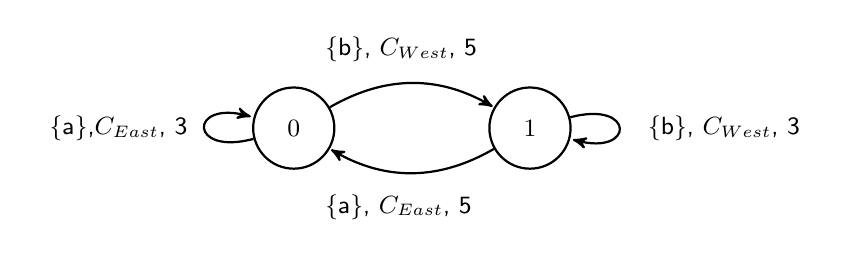
\begin{tikzpicture}[->,>=stealth',shorten >=0.5pt,auto,node distance=3cm,
                    thick,main node/.style={circle,draw,font=\sffamily\small}, align=center, text width=2cm]

  \node[main node, text width=0.7cm] (1) {$0$};
  \node[main node, text width=0.7cm] (2) [right of=1] {$1$};

  \node[align=left,font=\sffamily\small] (A) at (-2.1,0) {\{a\},$C_{East}$, 3};
  \node[align=left,font=\sffamily\small] (B) at (5.5,0) {\{b\}, $C_{West}$, 3};
  \node[align=left,font=\sffamily\small] (D) at (1.4,1) {\{b\}, $C_{West}$, 5};
  \node[align=left,font=\sffamily\small] (E) at (1.4,-1) {\{a\}, $C_{East}$, 5};
  \path[every node/.style={font=\sffamily\small}]
    (1) edge [bend left] node [above,sloped] {} (2)
        edge [loop left] node { } (1)
    (2) edge [bend left] node [below,sloped] {} (1)
        edge [loop right] node { } (2);
\end{tikzpicture}
\end{filecontents*}
\begin{figure}[htb]
\centering
\resizebox{9cm}{!}{ \begin{tikzpicture}[>=latex,shorten >=1pt,node distance=3cm,on grid,auto, node/.style={circle,draw,minimum size=25pt}, ]

 \node[state] (B) at (80pt,0pt) {$s_1$};

 \node[state] (A) at (0pt,0pt) {$s_0$};
 \draw[<-] (A) -- node[above left] {} ++(-1,0);
 \draw[->] (B) to[out=20,in=-20,looseness=8] node[right, align=left] {pass, 1} (B);
 \draw[->] (A) to[out=20,in=160,looseness=1] node[above] {snapshot, 0} (B);
 \draw[->] (B) to[out=200,in=-20,looseness=1] node[below] {move, 0} (A);
 \draw[->] (A) to[out=70,in=110,looseness=8] node[above left, align=left] {move, 2 \\ pass, 0} (A);


 \end{tikzpicture}
}
\caption{East-West soft constraint automaton}\label{fig:myfigure}
\end{figure}
\subsection{Soft Constraint Formula}
\paragraph{Syntax} Syntax. \\
Terms are ports and memory cells. 

\paragraph{Example} Example. \\
Given the soft constraint automaton $A$ above, its soft constraint formula is :

\begin{align*}
\phi(A) =  & \quad ( a \not = * \land b = * \land C_{East} \land 3_\mathbb{W} \land s=0 ) \lor (a = * \land b \not = * \land s=0 \land C_{West} \land s'=1 \land 5_\mathbb{W}) \lor \\
		 & \quad (a = * \land b \not = *  \land s=1 \land C_{West} \land 3_\mathbb{W}) \lor (a \not = * \land b = * \land s=1 \land C_{East} \land s'=0 \land 5_\mathbb{W}) \\
\end{align*}

\paragraph{Remark} Remark. \\
Each clause is a transition of the one state automaton derived from the constraint automaton.

\section{Compilation and Runtime}
Predictability and Robustness are two main challenges involve at Soft Component System runtime.

\subsection{Predictability}
Semiring values make the system deterministic by defining an ordering over the compiled transitions.

\paragraph{Algorithm} Chose transition at runtime \\
Semiring values define an order over a subsets of transition enabled for each system's configurations.


\subsection{Robustness}
Compile the transitions to a rewrite system. Prove properties on the rewrite system.
\subsubsection{Compilation to Maude}
\paragraph{Definition} Terms of the rewrite system \\
Ports and memory cells are defined in separated functional modules.
\begin{lstlisting}[style=base] 
	op p : Nat Data* -> Fact [ctor] . *** port of the protocol
	op q : Nat Data* -> Fact [ctor] . *** port of the environment
	op m : Nat Data* -> Fact [ctor] .
\end{lstlisting}

\paragraph{Definition} Rules of the rewrite system \\
Each clause is a rewrite rule where the left hand side consists of all the variables involved in the rule, and the right hand side consists of the all the variables involved in the rules with their updated data value.

\paragraph{Example} Alternator \\

\begin{lstlisting}[style=base]
	rl [3] : m(1,d_m1) p(3,*) => p(3,d_m1) m(1,*)  .
	rl [1] : m(1,*) m(2,d_m2) => m(1,d_m2) m(2,*)  .
	rl [4] : m(2,*) m(3,d_m3)  => m(2,d_m3) m(3,*)  .
	rl [2] : m(1,*) m(2,*) m(3,*) p(1,d_1) p(2,d_2) p(3,*) p(5,d_5) p(7,d_7) =>
		 p(1,*) p(2,*) p(3,d_1) p(5,*) p(7,*) m(1,d_2) m(2,d_5) m(3,d_7)  .

	eq startc = *** initialisation of mem cells, ports data. Link between port of 
			the protocol and the environment.
\end{lstlisting}

\paragraph{Definition} Trace module \\
Each input port and output port add its data to the trace module. The trace represents the observable behavior of the Soft Constraint System
\begin{lstlisting}[style=base] 
	op step : String Value -> Step [ctor] .
	op trace : StepList -> Fact [ctor] .
\end{lstlisting}

\paragraph{Definition} Environment module \\
The environment has two rewrite rules. If the environment port is linked with an input port of the protocol, the first rule produces data.  If the environment port is linked with an output port, the second rule consumes data.
\begin{lstlisting}[style=base] 
	op pg : Nat -> Data* .
	op counter : Nat Nat -> Fact .

	vars i j : Nat .
	var n : Nat .
	var k : Nat .
	var d : Data .
	
	eq pg(n) = string(n,10) .
	
	rl [prod] : in(i) link(i,j) q(j,k,*) => in(i) link(i,j) q(j,s k,pg(k)) .
	rl [cons] : out(j) link(i,j) q(i,k,d) => out(j) link(i,j) q(i,k,*) .
\end{lstlisting}

\paragraph{Definition} Runtime module \\
The environment has two rewrite rules. If the environment port is linked with an input port of the protocol, the first rule produces data.  If the environment port is linked with an output port, the second rule consumes data.
\begin{lstlisting}[style=base] 
	vars i j : Nat .
	var k : Nat .
	var d : Data .

	rl [ruleOut] : link(i,j) out(i) p(i,d) q(j,k,*) => link(i,j) out(i) p(i,*) q(j,k,d). 
	rl [ruleIn] : link(i,j) in(i) p(i,*) q(j,k,d) => link(i,j) in(i) p(i,d) q(j,k,*) . 
\end{lstlisting}


\subsubsection{property analysis}


\/*
If all actions are components, can we consider rewriting port data stream only in Maude ? \\
Could we define a special data item to say if a port is ready and build conditional rewrite rules regarding this item ? \\
We can prove properties on traces of our system. Could we use the trace of a "log" component synchronized on each actions to prove properties ?
*/

\/*
\paragraph{State Transition representation of Soft Component Automaton} \hspace{0pt} \\

\begin{filecontents*}{temp.tikz}
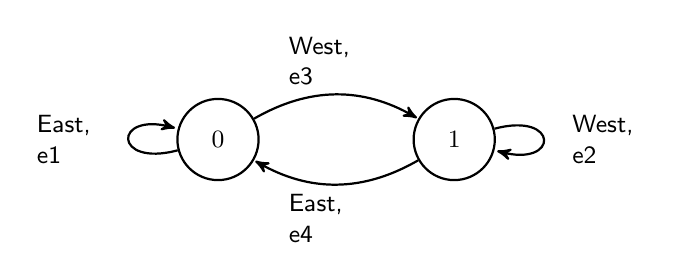
\begin{tikzpicture}[->,>=stealth',shorten >=0.5pt,auto,node distance=3cm,
                    thick,main node/.style={circle,draw,font=\sffamily\small}, align=center, text width=1cm]

  \node[main node, text width=0.7cm] (1) {$0$};
  \node[main node, text width=0.7cm] (2) [right of=1] {$1$};

  \node[align=left,font=\sffamily\small] (A) at (-1.8,0) {East, e1};
  \node[align=left,font=\sffamily\small] (B) at (5,0) {West, e2};
  \node[align=left,font=\sffamily\small] (D) at (1.4,1) {West, e3};
  \node[align=left,font=\sffamily\small] (E) at (1.4,-1) {East, e4};
  \path[every node/.style={font=\sffamily\small}]
    (1) edge [bend left] node [above,sloped] {} (2)
        edge [loop left] node { } (1)
    (2) edge [bend left] node [below,sloped] {} (1)
        edge [loop right] node { } (2);
\end{tikzpicture}
\end{filecontents*}

\begin{figure}[htb]
\centering
\resizebox{9cm}{!}{ \begin{tikzpicture}[>=latex,shorten >=1pt,node distance=3cm,on grid,auto, node/.style={circle,draw,minimum size=25pt}, ]

 \node[state] (B) at (80pt,0pt) {$s_1$};

 \node[state] (A) at (0pt,0pt) {$s_0$};
 \draw[<-] (A) -- node[above left] {} ++(-1,0);
 \draw[->] (B) to[out=20,in=-20,looseness=8] node[right, align=left] {pass, 1} (B);
 \draw[->] (A) to[out=20,in=160,looseness=1] node[above] {snapshot, 0} (B);
 \draw[->] (B) to[out=200,in=-20,looseness=1] node[below] {move, 0} (A);
 \draw[->] (A) to[out=70,in=110,looseness=8] node[above left, align=left] {move, 2 \\ pass, 0} (A);


 \end{tikzpicture}
}
\caption{Soft Component Automaton \textit{A}}\label{fig:myfigure}
\end{figure}


\paragraph{Logical representation of Soft Component Automaton} \hspace{0pt}\\
 
\textbf{Syntax.}The syntax of a formula $\phi \in L$ is as follows : 
$$\phi:= \quad e \quad | \quad t_1=t_2 \quad |\quad R(t_1, .. ,t_n) \quad | \quad \phi_1 \land \phi_2 \quad | \quad \neg \phi \quad | \quad \exists x \phi \quad  $$ where $e \in \mathbb{E}$.

Given that $A'_i$ is the action $A_i$ in conjunction with the state constraints, the logical expression of A is:
\begin{align*}
\phi(A) =  & \quad ( s=0 \land A_1 \land s'=0 \land e_{1}) \lor (s=0 \land A_2 \land s'=1 \land e_{3}) \lor (s=1 \land A_2 \land s'=1 \land e_{2}) \lor (s=1 \land A_1 \land s'=3 \land e_{4}) \\
		=  & \quad ( A'_1 \land e_{1}) \lor ( A'_2 \land e_{3}) \lor (A'_2 \land e_{2}) \lor ( A'_1 \land e_{4}) \\
		=  & \quad  ( \text{down}(0,1) \land 5_\mathbb{W} \lor \text{up}(0,0) \land 3_\mathbb{W} \lor \\
		& \quad \text{ down(1,1)} \land 3_\mathbb{W} \lor  \text{up(1,0)} \land 5_\mathbb{W})\\
		=  & \quad  (\text{listen} \land 2_\mathbb{W} \lor  \\
		&  \quad \text{ emit} \land 1_\mathbb{W})\\
		=  & \quad   \text{down(0,1)}\land \text{listen} \land 10_\mathbb{W} \lor \text{up(0,0)}\land \text{emit} \land 3_\mathbb{W} \lor \\
			& \quad \text{down(1,1)}\land \text{listen} \land  6_\mathbb{W} \lor  \text{up(1,0)}\land \text{emit} \land 5_\mathbb{W}
\end{align*}
\/*
Let's remark that $\phi(A)$ can be interpreted as a semiring value : 

$\top=0_\mathbb{W}$
$\bot=\infty_\mathbb{W}$
\textbf{Semantics.}The semantic is defined by $\llbracket . \rrbracket$ as follow : \\
\/*
$$\frac{e \in L}{\llbracket e \rrbracket \in \mathbb{E}} \quad \quad \frac{e \in L}{\llbracket e \rrbracket \in \mathbb{E}}$$
$$\frac{e \in L}{\llbracket e \rrbracket \in \mathbb{E}} \quad \quad \frac{e \in L}{\llbracket e \rrbracket \in \mathbb{E}}$$

\begin{align*}
\llbracket e \rrbracket =  & \quad e \in \mathbb{E} \\
\llbracket t_1=t_2 \rrbracket =  & \quad 1_\mathbb{B} \quad |\quad 0_\mathbb{B} \quad \in \mathbb{B} \\
\llbracket \phi \land \psi \rrbracket =  & \quad \llbracket \phi \rrbracket  \otimes \llbracket \psi \rrbracket \\
\llbracket \phi \lor \psi \rrbracket =  & \quad \llbracket \phi \rrbracket  \oplus \llbracket \psi \rrbracket \\
\llbracket \neg \phi \rrbracket =  & \quad 1_\mathbb{B} - \llbracket \phi \rrbracket \quad  \text{if $\phi$ has a binary semiring valuation}
\end{align*}
where $\otimes$ and $\oplus$ are two polymorphic operators. By polymorphic, this operator is interpreted regarding the type of the two operands semiring values. At this point, we assume that the evaluation of this operator is given for any possible composition of semiring values. The formula describing A can be interpreted as follow:
\begin{align*}
\llbracket \phi(A) \rrbracket =  & \quad \llbracket( A'_1 \land e_{1})\rrbracket \oplus \llbracket( A'_2 \land e_{3})\rrbracket \oplus \llbracket(A'_2 \land e_{2})\rrbracket \oplus \llbracket( A'_1 \land e_{4})\rrbracket \\
					=  & \quad (\llbracket A'_1\rrbracket \otimes \llbracket e_{1}\rrbracket) \oplus (\llbracket A'_2\rrbracket \otimes \llbracket e_{3}\rrbracket) \oplus (\llbracket A'_2\rrbracket \otimes \llbracket e_{2}\rrbracket) \oplus (\llbracket A'_1\rrbracket \otimes \llbracket e_{4}\rrbracket)
\end{align*}
In this example, $A_1$ is a binary constraint, and is evaluated to $1_\mathbb{B}$ or to $0_\mathbb{B}$. The composition operator is define over $\mathbb{E}\times\mathbb{E}$ with any semiring $\mathbb{E}$. If it operates over $\mathbb{B}\times\mathbb{E}$, we can still interpret this operator over $\mathbb{E}\times\mathbb{E}$ by applying homomorphic transformation $h_\mathbb{E}:\mathbb{B} \to \mathbb{E}$ with $h_\mathbb{E}(0_\mathbb{B})=0_\mathbb{E}$ and $h_\mathbb{E}(1_\mathbb{B})=1_\mathbb{E}$. Assuming that $e_i \in \mathbb{E}$,  
\begin{align*}
\llbracket \phi(A) \rrbracket =  & \quad (h_\mathbb{E}(\llbracket A'_1\rrbracket) \otimes \llbracket e_{1}\rrbracket) \oplus (h_\mathbb{E}(\llbracket A'_2\rrbracket) \otimes \llbracket e_{3}\rrbracket) \oplus (h_\mathbb{E}(\llbracket A'_2\rrbracket) \otimes \llbracket e_{2}\rrbracket) \oplus (h_\mathbb{E}(\llbracket A'_1\rrbracket) \otimes \llbracket e_{4}\rrbracket)
\end{align*}
Polymorphic operators are interpreted regarding the type of the semiring involved in the product. $T_{\mathbb{E}}$ is the type of the semiring $\mathbb{E}$ and the polymorphic operators are : 
$$\otimes_{T_{\mathbb{E}_1} \times T_{\mathbb{E}_2}} : \mathbb{E}_1 \times \mathbb{E}_2 \to \mathbb{E}_3$$ 
\/*
$$\oplus_{\mathbb{E}_1 \times \mathbb{E}_2} : \mathbb{E}_1 \times \mathbb{E}_2 \to \mathbb{E}_3$$ 
\/*
where $\mathbb{E}_i$ are either atomic semirings (weighted, probabilistic, .. ) or a product of atomic semirings. As an example, $T_{\mathbb{E}_1}$ could be the Energy semiring and $ T_{\mathbb{E}_2}$ the Time semiring and interpret $\otimes$ as

\textbf{Composition.} Let A and B be two automata with only one transition $\phi_i$ and one semiring value $e_i$. We want to get the product of those two automata, according to their semiring preference. The composition operator is polymorphic at the level of automata composition, and is interpreted with the right and left hand side type of semiring value. 
\begin{align*}
& \phi(A) =   \phi_1 \land e_1 
& \phi(B) =   \phi_2 \land e_2
\end{align*}
\begin{align*}
A \odot B \equiv \quad \phi(A) \land \phi(B) & = \phi_1 \land e_1 \land \phi_2 \land e_2
\end{align*}
\begin{align*}
\oplus (A \odot B) \equiv \quad \llbracket \phi(A) \land \phi(B) \rrbracket  & = \llbracket \phi_1 \land e_1 \land \phi_2\land e_2 \rrbracket \\
& = \llbracket \phi_1 \rrbracket \otimes e_1 \otimes \llbracket \phi_2 \rrbracket \otimes e_2 
\end{align*}

\paragraph{Domain of a composed semiring value :} \hspace{0pt} \\
Semiring elements are maps from semiring type to value. The composition operator is the composition of the semiring in the intersection of the two maps, and the union of both fields otherwise. Let's take an example :
\begin{align*}
& e_1 =   \{\text{energy : 5 ; space : 4}\} 
& e_2 =   \{\text{energy : 3 ; time : 0.1}\} \\
& \text{energy} \otimes \text{energy} = \text{energy} \odot \text{energy} \\
& \text{space} \otimes \text{time} = \text{space} \triangleright \text{time} 
\end{align*}
The jion composition of $e_1$ and $e_2$ is :
\begin{align*}
 e_1 \otimes e_2 = \quad  & \{\text{energy : } 5 \otimes 3 \text{ ; space}\triangleright \text{time ;  : 4} \triangleright \text{0.1}\} \\
 		= \quad & \{\text{energy : } 15 \text{ ; space}\triangleright \text{time ;  : 4} \triangleright \text{0.1}\}
\end{align*}
*/
\/*
\paragraph{ Coproduct Semiring} \hspace{0pt} \\
Define the semiring where the product belongs as a coproduct.
*/




\/*
The semiring value of this formula is :
Composition :
\begin{align*}
A \odot B \equiv & \quad \phi(A) \land \phi(B) \land E'_A=join_A(E_A,E_B) \land E'_B = join_B(E_A,E_B) \\
		=  & \quad [\bigvee_i(A'_i \land m_{A}=e_{A_i})] \land m_A'= (\oplus_A E_A) \land E_A'= \cup_{A_i} \{ e_{A_i} \otimes f(A'_i)\}  \land \\
		& \quad  [\bigvee_i(B'_i \land m_{B}=e_{B_i})] \land m_B'= (\oplus_B E_B) \land E_B'= \cup_{B_i} \{ e_{B_i} \otimes f(B'_i)\} \land  \\
		& \quad E'_A=join_A(E_A,E_B) \land E'_B = join_B(E_A,E_B) \\
\end{align*}

\paragraph{Semiring representation of Soft Component Automaton} \hspace{0pt} \\


\/*
\noindent
To declare a Soft Constraint Automata within REO semantics, the name of the semirings, its parameters (such as its value and threshold) appear in the signature. Then, $A0<energyW<x,y>>(){}$ defines the automata A0 with energyW an instance of the underlying semiring energy, x the preference value given for this semiring, and y the threshold. As soon as the name of each instantiation is unique, this model lets us access to all semiring of the automata.
\begin{lstlisting}[frame=single,style=base] 
A0<energyW@<2>@,@t=1@>(){
    energy : {W}
    @t : energy@

    q0 -> q0 : {a,b}, a>b, energyW:{energy} 

 }
\end{lstlisting}
\begin{lstlisting}[frame=single,style=base] 
A1<moodH@<3>@,moodS@<2>@,constH@<0.2>@,constS@<0.7>@,@t=<0.1,1>@>(){
    mood : {W}; const : {P}
    @t : <const,mood>@

    q1 -> q1 : {b,c}, b<c , constS:{const}
    q1 -> q2 : {b,c}, b>c , moodH:{mood}
    q2 -> q1 : {b,c}, b<c , moodS:{mood}
    q2 -> q2 : {b,c}, b>c , constH:{const}

}
\end{lstlisting}
\paragraph{Composed Soft Constraint Automata into REO semantic} \hspace{0pt}\\
Automata $A_0$ and $A_1$ can be composed to obtain a new automata $A_0.A_1$ as displayed below:
\begin{filecontents*}{temp.tikz}
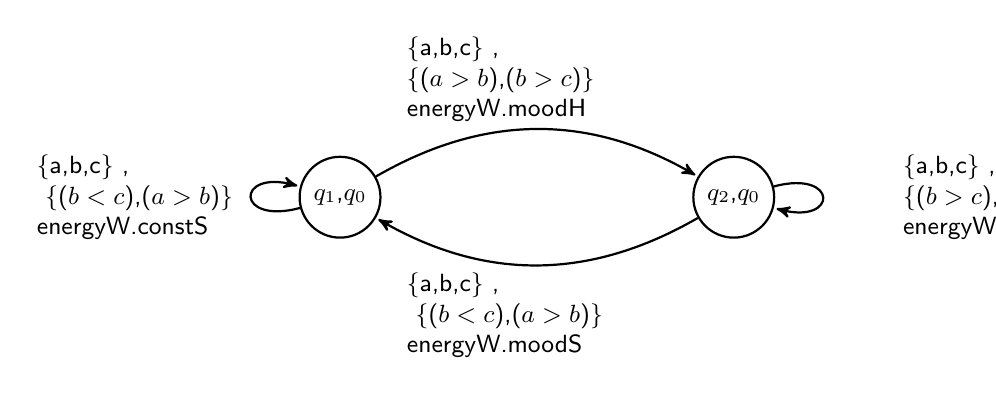
\begin{tikzpicture}[->,>=stealth',shorten >=1pt,auto,node distance=5cm,
                    thick,main node/.style={circle,draw,font=\sffamily\small}, align=center, text width=0.7cm]

  \node[main node] (1) {$q_1$,$q_0$};
  \node[main node] (2) [right of=1] {$q_2$,$q_0$};
  
\iffalse
  \node[main node] (4) [below right of=1] {4};
\fi

  \node[align=left,font=\sffamily\small] (A) at (-3.5,0) {\text{\{a,b,c\} ,} \\ \text{ \{($b<c$),($a>b$)\}} \\ \text{energyW.constS}};
  \node[align=left,font=\sffamily\small] (A) at (7.5,0) {\text{\{a,b,c\} ,} \\ \text{\{($b>c$),($a>b$)\}} \\ \text{energyW.constH}};
  \node[align=left,font=\sffamily\small] (A) at (1.2,1.5) {\text{\{a,b,c\} ,} \\ \text{\{($a>b$),($b>c$)\}} \\ \text{energyW.moodH}};
  \node[align=left,font=\sffamily\small] (A) at (1.2,-1.5) {\text{\{a,b,c\} ,} \\ \text{ \{($b<c$),($a>b$)\}} \\ \text{energyW.moodS}};
  \path[every node/.style={font=\sffamily\small}]
    (1) edge [bend left] node [above,sloped] {} (2)
        edge [loop left] node { } (1)
    (2) edge [bend left] node [below,sloped] {} (1)
        edge [loop right] node { } (2);
\end{tikzpicture}
\end{filecontents*}
\begin{figure}[htb]
\centering
\resizebox{14cm}{!}{ \begin{tikzpicture}[>=latex,shorten >=1pt,node distance=3cm,on grid,auto, node/.style={circle,draw,minimum size=25pt}, ]

 \node[state] (B) at (80pt,0pt) {$s_1$};

 \node[state] (A) at (0pt,0pt) {$s_0$};
 \draw[<-] (A) -- node[above left] {} ++(-1,0);
 \draw[->] (B) to[out=20,in=-20,looseness=8] node[right, align=left] {pass, 1} (B);
 \draw[->] (A) to[out=20,in=160,looseness=1] node[above] {snapshot, 0} (B);
 \draw[->] (B) to[out=200,in=-20,looseness=1] node[below] {move, 0} (A);
 \draw[->] (A) to[out=70,in=110,looseness=8] node[above left, align=left] {move, 2 \\ pass, 0} (A);


 \end{tikzpicture}
}
\caption{$A_0.A_1$ is the composition between $A_0$ and $A_1$}\label{fig:myfigure}
\end{figure}

\newpage
\noindent
REO semantics for the composed automata :
\begin{lstlisting}[frame=single,style=base] 
//As it should be for composing A0 and A1 :
A2 = A0<2,t=1>.A1<3,1,0.2,0.7,t=(1,0.1)>

// Which gives :
A2 = A0.A1<energyW.constS@<2,0.7>@,energyW.constH@<2,0.2>@,energyW.moodS@<2,2>@,
           energyW.moodH@<2,3>@,@t=<(1,1),(1,0.1)>@>(){
    energy : {W}
    const : {P}
    @t : <energy.mood,energy.const>@

    (q1,q0) -> (q2,q0) : {a,b,c}, {(a>b),(b>c)}, energyW.moodH:{energy.mood}
    (q1,q0) -> (q1,q0) : {a,b,c}, {(a>b),(b<c)}, energyW.constS:{energy.const}
    (q2,q0) -> (q2,q0) : {a,b,c}, {(a>b),(b>c)}, energyW.constH:{energy.const}
    (q2,q0) -> (q1,q0) : {a,b,c}, {(a>b),(b<c)}, energyW.moodS:{energy.mood}

 }
\end{lstlisting}
\iffalse
    (1) edge node [left] {0.6} (4)
        edge [bend right] node[left] {0.3} (2)
        edge [loop above] node {0.1} (1)

    (2) edge node [right] {0.4} (1)
        edge node {0.3} (4)
        edge [loop left] node {0.4} (2)
        edge [bend right] node[left] {0.1} (3)

    (3) edge node [right] {0.8} (2)
        edge [bend right] node[right] {0.2} (4)

    (4) edge node [left] {0.2} (3)
        edge [loop right] node {0.6} (4)
        edge [bend right] node[right] {0.2} (1);
    Define styles for edges, arrows, and nodes
        circle style for the main nodes, and font options so we don't need to adjust fonts within the nodes
        For arrows, we use stealth' which is the name for a kind of arrow tip and shorten to not touch the node
        The option auto is useful for automatic placement of nodes next to edges, instead of sitting directly on the edge. As we will mostly use left and right options, it will have effect just for one node. But good to have it as general option in the scope.
    Place the main nodes
    Draw edges with nodes for description
    Use options loop and bend for loops and bent edges
    Specify left and right for bend direction and node placement
\fi
*/

\end{document}


